\documentclass[12pt]{exam}
\usepackage[utf8]{inputenc}
\usepackage{graphicx}

\graphicspath{{DickPick/}}


\begin{document}

\begin{questions}
\question \textbf{Décrire ce que fait ce programme très simple en un paragraphe.}

Ce programme début en initialisant un thread avec la fonction led\_thread et par la suite entre dans la boucle principale. Cette boucle attend 1 seconde (1000ms) et ensuite signal le thread 1 avec le signal 0x1. Ce signal permet alors au led\_thread d'exécuter ses fonctions. Il ajout + 1 a i et j et il change l'étât dans lequel la led1 était.

\question \textbf{Placer un point d’arrêt à une position vous permettant de suivre l’évolution des valeurs de i et de j durant l’exécutiondu programme. Donner une copie d’écran montrant le positionnement de ce point d’arrêt.}
\par
\centering
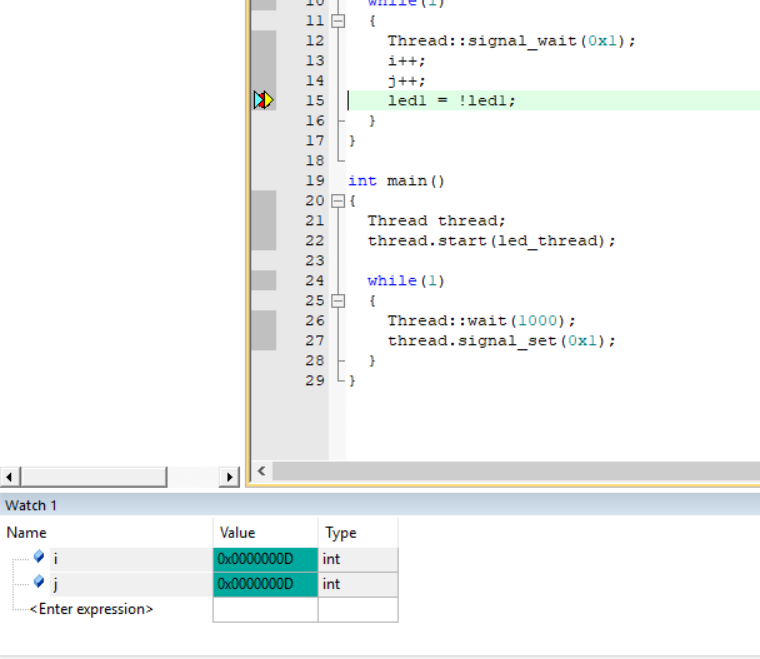
\includegraphics[scale=0.5]{no2}
\end{questions}
\end{document}